\documentclass[a4paper,10pt]{article}
\usepackage[margin=15mm]{geometry}
\usepackage{pgf,tikz}
\usepackage{subfig}
\usepackage{amsmath}
\usepackage{color}
\usepackage{amssymb}
\usepackage{noweb}
\usepackage{listings}
\usetikzlibrary{circuits.logic.US}
\usetikzlibrary{positioning}
\usetikzlibrary{matrix}
 
\definecolor{dkgreen}{rgb}{0,0.6,0}
\definecolor{gray}{rgb}{0.5,0.5,0.5}
\definecolor{mauve}{rgb}{0.58,0,0.82}

\lstset{ %
  language=Verilog,                % the language of the code
  basicstyle=\footnotesize,           % the size of the fonts that are used for the code
  numbers=left,                   % where to put the line-numbers
  numberstyle=\tiny\color{gray},  % the style that is used for the line-numbers
  stepnumber=2,                   % the step between two line-numbers. If it's 1, each line 
                                  % will be numbered
  numbersep=5pt,                  % how far the line-numbers are from the code
  backgroundcolor=\color{white},      % choose the background color. You must add \usepackage{color}
  showspaces=false,               % show spaces adding particular underscores
  showstringspaces=false,         % underline spaces within strings
  showtabs=false,                 % show tabs within strings adding particular underscores
%  frame=single,                   % adds a frame around the code
  rulecolor=\color{black},        % if not set, the frame-color may be changed on line-breaks within not-black text (e.g. commens (green here))
  tabsize=2,                      % sets default tabsize to 2 spaces
  captionpos=b,                   % sets the caption-position to bottom
  breaklines=true,                % sets automatic line breaking
  breakatwhitespace=false,        % sets if automatic breaks should only happen at whitespace
  title=\lstname,                   % show the filename of files included with \lstinputlisting;
                                  % also try caption instead of title
  keywordstyle=\color{blue},          % keyword style
  commentstyle=\color{dkgreen},       % comment style
  stringstyle=\color{mauve},         % string literal style
  escapeinside={\%*}{*)},            % if you want to add LaTeX within your code
  morekeywords={*,...}               % if you want to add more keywords to the set
}
\usepackage{amsthm}
\usepackage{hyperref}
\setlength{\parskip}{3mm}
\newtheorem{axiom}{Axiom}
\newtheorem{definition}{Definition}
\newtheorem{comment}{Comment}
\newtheorem{example}{Example}
\newtheorem{lemma}{Lemma}
\newtheorem{prop}{Property}
\newtheorem{problem}{Problem}
\newtheorem{remark}{Remark}
\newtheorem{theorem}{Theorem}

% Title Page
\title{Introduction to VHDL}
\author{Dilawar Singh}
\date{\today}

\begin{document}
\maketitle

\begin{abstract}
  
  This is not a tutorial of VHDL language. A minimal familiarity with grammar of
  computer languages are assumeed. It has been assumed that you have read the
  document posted on moodle about \textbf{proto-rtl} language.

\end{abstract}

\section{Introduction}
  
  Consider the following piece of hardware.
 
  \begin{figure}[h]
    \input{/home/dilawar/Scripts/tikz/circuit_macros.tex}
    \begin{center}
      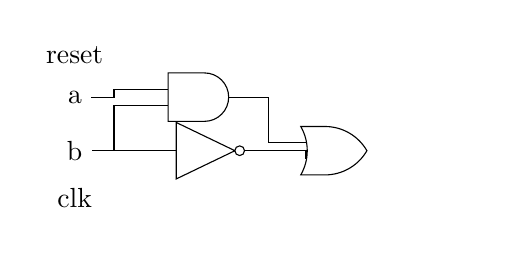
\begin{tikzpicture}[circuit logic US]
        %\dflipflop{(c.center)}{2}{2}{``DFF''};
        %% Draw the combinational logic.
        \matrix[column sep=7mm]
        {
          \node (reset) {reset}; & & & & \\
          \node (a) {a}; & \node[and gate] (a1) {}; &  & & \\ 
          \node (b) {b};  & \node[not gate] (n1) {};& \node[or gate] (o1) {}; & & \\
          \node (clk) {clk};  &  & & \\
        };
        % \dflipflop{(clk)}{1}{1}{dff};
        % \draw (reset) -| (dff_reset);
        \draw (a) -- ++(right:5mm) |- (a1.input 1);
        \draw (b) -- ++(right:5mm) |- (a1.input 2);
        \draw (b) -- ++(right:5mm) |- (n1.input);
        \draw (n1.output) -| (o1.input 2);
        \draw (a1.output) -- ++(right:5mm) |- (o1.input 1);
      \end{tikzpicture}
    \end{center}
    \caption{A small toy circuit. Describe it in proto-RTL.}
    \label{fig:circuit}
  \end{figure}

\end{document}          
